% !TEX encoding = UTF-8 Unicode
% !TEX root = ../thesis.tex
% !TEX spellcheck = en-US
%%=========================================



\chapter{Implementation}

% Hololens, UWP, WMR


% and non-functional requirements, which describe  

\section{Development}
This research project has been in active progression for two semesters and development has effectively been done in two stages. First in October and November 2020 and then from February till May in 2021. During the fall and first stage of development the focus was on the HoloLens 2 and creating a usable act of dissection in augmented reality. The second stage at spring, had a wider scope, with focus on implementing networking, volumetric data and more. During this chapter it will thus be clearly discrete improvements during the first iterations of the product while later iterations will be grouped and focus will be put on specific features or pain points. The final iteration will focus on improvements done from user feedback and the feature set at the end of development.

\subsection[Iteration 0]{Iteration 0: First steps, importing model}\label{chap:zeroiter}
% 0th iteration: Initializing application, importing and simplifying brain model

\begin{wrapfigure}{r}{0.45\textwidth} 
    \centering
    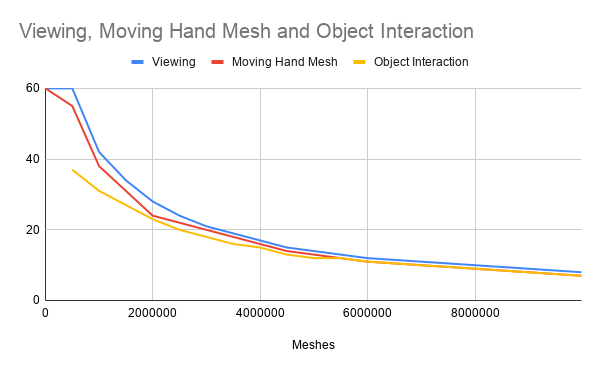
\includegraphics[width=0.45\textwidth]{fig/hololens2polycount}
    \caption{Figure showing frame rate as a function of polygon count on HoloLens 2. Credit: \href{https://community.fologram.com/t/hololens-2-polygon-count-and-frame-rate/49}{Fologram}}
    \vspace{20pt}
    \label{fig:polycount}
\end{wrapfigure}

The first phase of development started by acquiring the surface model of the WHS rat brain created by \citet{Elden2017}. This was done by simply moving the FBX files from the \nameref{chap:vrvis} application and to a new Unity project. After initializing MRTK by following their \href{https://microsoft.github.io/MixedRealityToolkit-Unity/version/releases/2.2.0/Documentation/GettingStartedWithTheMRTK.html}{Getting Started documentation}, the application was ready to deploy on the HoloLens 2. This resulted in a barely running application as the polygon count of the brain model was orders of magnitude larger than what is recommended to maintain adequate performance on the HoloLens 2, which is in the order of 100,000 polygons shown in \autoref{fig:polycount}. The model used by Elden was scaled to run on workstation computer outputting to an HTC Vive, and thus his model was reduced from a original 16 million polygons to around 3 million. The HoloLens 2 runs all calculations on-device on a mobile ARM-based processing unit and naturally the brain model created for rendering on a dedicated workstation graphics card had to be further scaled down. 
This downscaling was first experimented with doing at run-time dynamically on-device using the library \textit{UnityMeshSimplifier}. It was quickly determined that this was not a viable solution both because of untenable processing time, but also because the simplified result had a huge impact on quality of model, hinting at the performance optimization that had to be done on the simplifier algorithm to be able to execute at run-time. The next and final solution for downscaling was to use the \textit{decimate} modifier in \nameref{chap:blender}. \textit{Incremental decimation} is a mesh simplification algorithm which trades some speed for higher mesh quality, in contrast to the \textit{vertex clustering} presumably used in UnityMeshSimplifier which prioritizes speed in such a way that topology is not preserved. Within Blender functionality for simple application of the modifier to all objects in a tree-structure was not found, or understood to exist, so a script applying the decimate modifier with a given ratio was written, see \autoref{item:blenderscript}. The \texttt{ratio} parameter is a value between 0 and 1, representing the scaling of the resulting mesh' polygon count.

\begin{lstlisting}[language=python, label={item:blenderscript}, caption={Blender script applying a decimate modifier to all relevant objects in a scene.}]
import bpy # importing the blender python library

def decimate(ratio, replace = True):
    # Finds all objects and filters irrelevant objects from the FBX 
    brainparts = [n for n in bpy.data.objects \
        if n.name not in ("Camera", "Light")] 

    for part in brainparts:
        mod = part.modifiers.new(type='DECIMATE', name='Decimate')
        mod.decimate_type = 'COLLAPSE'
        # Sets the specifies strength to the decimate operation. 
        mod.ratio = ratio
# Calls function with given decimate strength.
decimate(0.08)
\end{lstlisting}

The resulting decimated model, even at the ratio of 0.08, was visibly nearly indistinguishable from the original model when looking at them through the HoloLens 2 display which, as described in \autoref{chap:hololens2}, is somewhat blurry. \autoref{fig:decimate} shows the difference as seen in the Unity editor. Ultimately, a decimation ratio of 0.08 was chosen as a compromise between detail and performance being about 300,000 polygons, this compromise will be discussed further in \autoref{chap:discussperformance}. At this stage requirement 1 and 2 in the initial requirements from \autoref{chap:req} could conclusively be answer as possible and completed.
\begin{figure}[ht]
    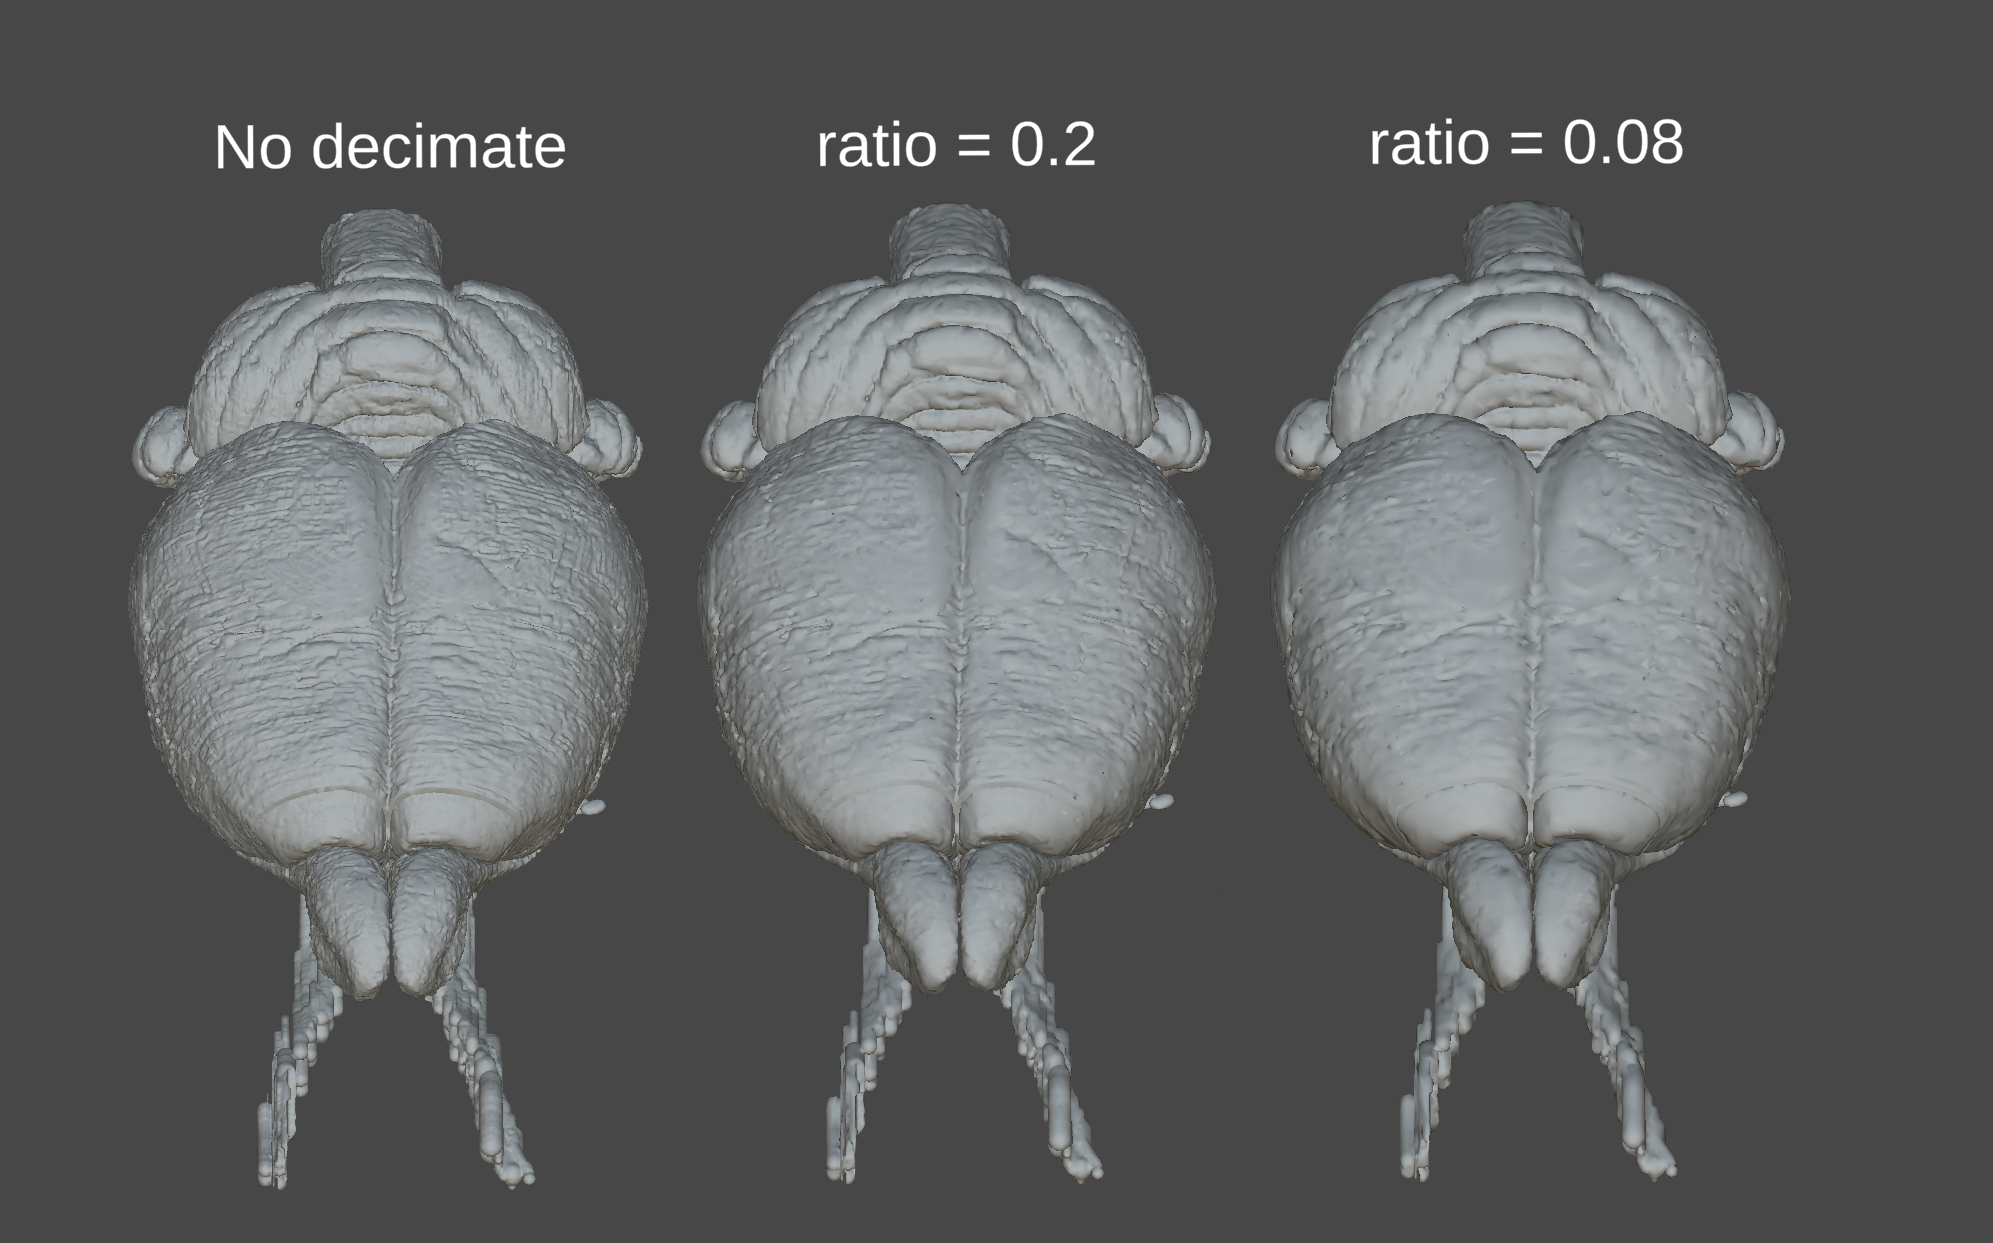
\includegraphics[width=\textwidth]{fig/brainmodeldecimateratio2.png}
    \caption{WHS rat brain models with decreasing polygon count.}
    \label{fig:decimate}
\end{figure}



\subsection[Iteration 1]{First iteration: Minimum Viable Product}\label{chap:itr1}

Having a surface model of the brain running reasonably well on the HoloLens 2, the next step in developing the application was to implement basic AR-based interact features. The brain model consist of an empty parent object with 29 children each containing the mesh of a delineated brain structure, see \autoref{fig:brainunitytree}. Adding the \texttt{Object Manipulator} component from MRTK and a standard Unity \texttt{Mesh Collider} component to each child in the brain model allows for picking apart the brain. This is done by grabbing and moving each separate structure with a MRTK defined \textit{pointer}, this is the logical abstraction for the simplest interact handling with HoloLens 2 giving the user a virtual laser pointer from their finger. The resulting action can be seen in \autoref{fig:grabbrain}. 

% \begin{wrapfigure}{r}{0.38\textwidth} 
%     \centering
%     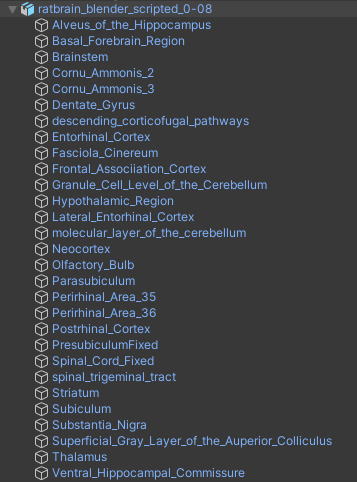
\includegraphics[width=0.35\textwidth]{fig/brainunitytree.png}
%     \caption{The tree structure of the Unity \texttt{GameObject} of the brain model.}
%     \vspace{-10pt}
%     \label{fig:brainunitytree}
% \end{wrapfigure}

\begin{figure}[ht]
    \centering
    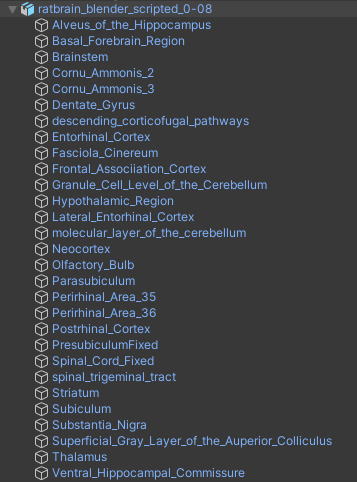
\includegraphics[width=0.30\textwidth]{fig/brainunitytree.png}
    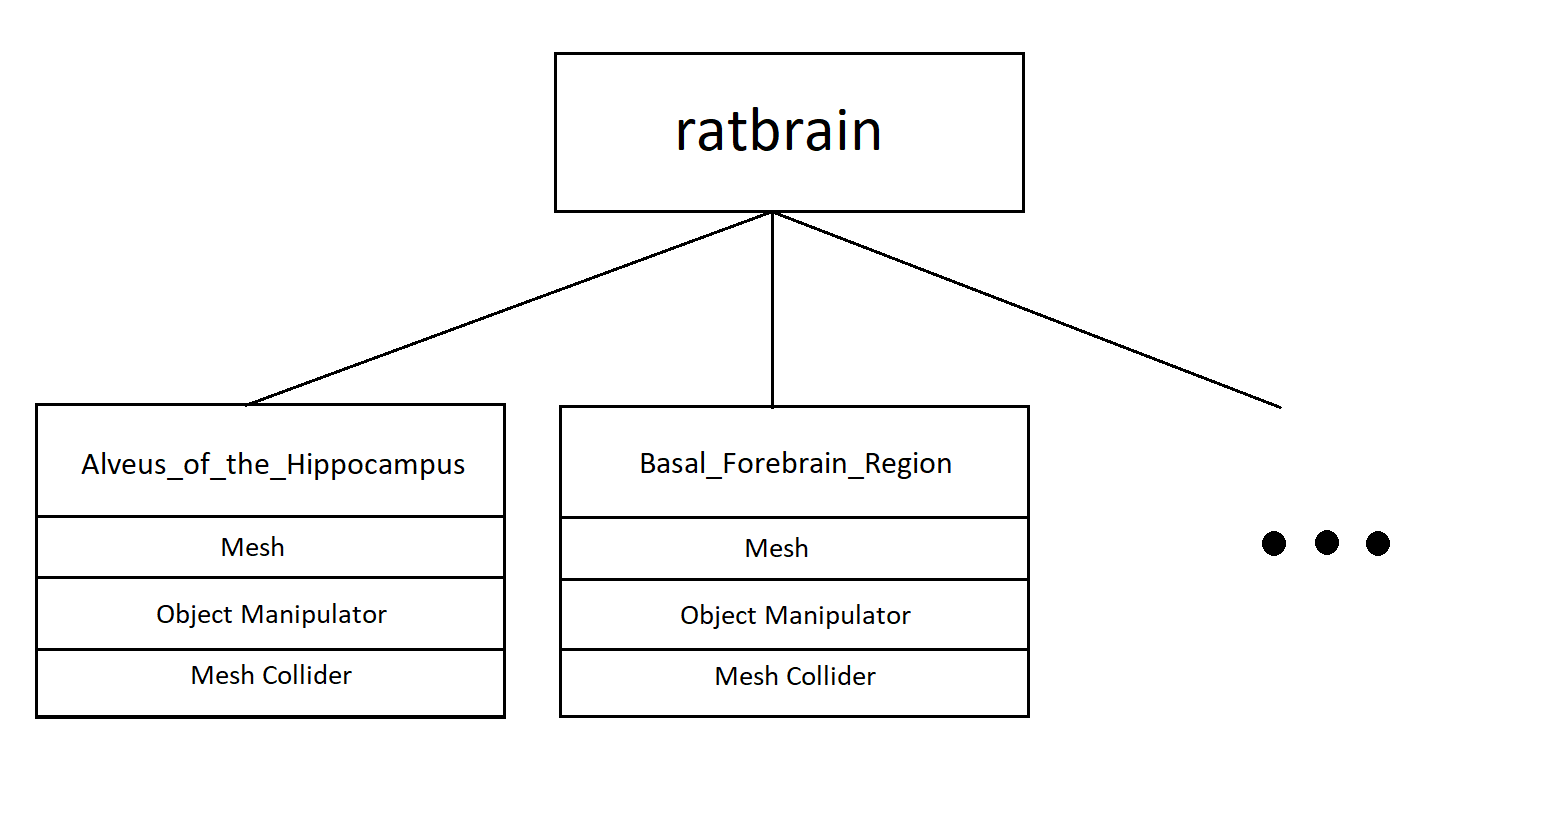
\includegraphics[width=0.60\textwidth]{fig/shittyassbraintreediagram.png}
    \caption{The tree structure of the Unity \texttt{GameObject} of the brain model.}
    \label{fig:brainunitytree}
\end{figure}

\begin{figure}[ht]
    \centering
    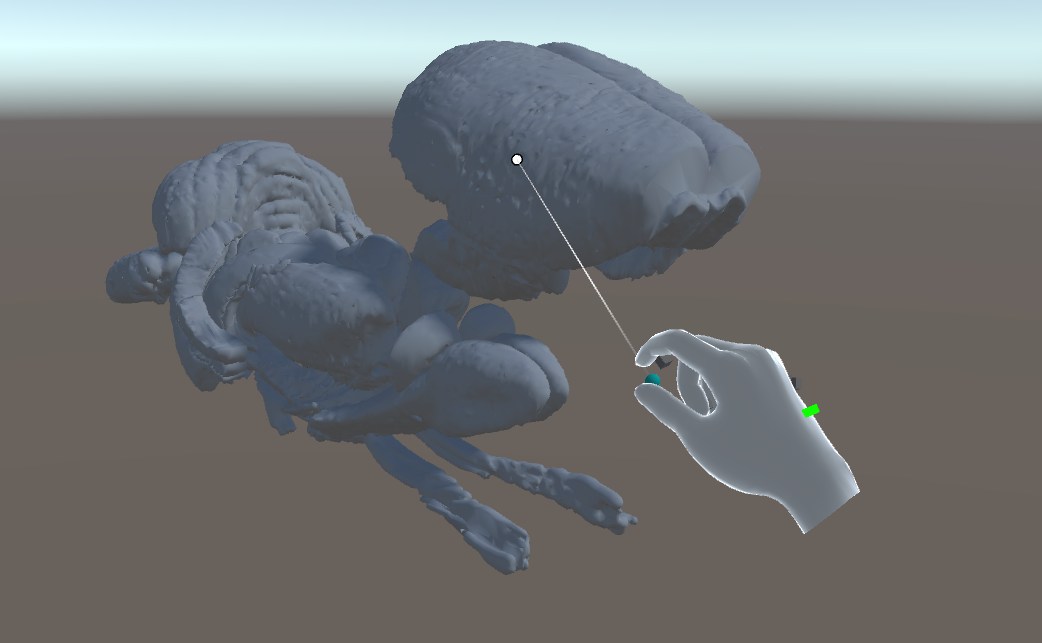
\includegraphics[width=0.8\textwidth]{fig/grabbrainsection.png}
    \caption{Grabbing the neocortex brain structure with a MRTK pointer in the Unity editor.}
    \label{fig:grabbrain}
\end{figure}

An apparent problem at this stage was that thought the brain structures are separate objects, they were difficult to visually distinguish from each other. A script which took all child objects and applied a random color to each was written and placed on the parent object, thus quickly giving some visual separation of the structures. While implementing this feature, the \textit{material} of each child was changed from Unity's default material to a \textit{MRTK Standard} material. Materials are the way Unity handles rendering details for each object, this is where shader, texture and general rendering options are configured. The MRTK Standard materials is a set of materials using the the \texttt{MixedRealityStandard.shader} shader, this shader is optimized for MR use, and superficially for HoloLens, and is meant for fulfill all shader-needs when developing for these platforms. 

% Jeg heter Ole og jeg har liten tiss

With a some basic visibility and manipulation features for the brain model, the next natural step was tackling the system requirements, specifically the first functional requirement, implementing brain dissection. A \textit{clipping} shader was written and implement to work with the brain, giving more control over the feature than using MRTKs prebuild clipping feature, but seeing as it was not possible to combine a custom shader with MRTK optimizes feature set for AR rendering, the custom clipping implementation was abandoned in favor of MRTK, using the aforementioned MixedRealityStandard shader. Clipping has the effect of removing vertices by some defined function, and by using a prebuilt clipping plane prefab and declare on which meshes is should act, a dissection affect was created. A handle for manipulating the plane was added for ease of use, by dragged a ball the plane would move such that it was a fixed distance from the ball and perpendicular to the line between the ball and the center of the brain. 


Further, a hovering menu displaying the name of the last grabbed brain structure and buttons for the actions moving, transparency and dissection was implemented. This was created by modifying a MRTK prefab and updating its name based on the name of the \texttt{GameObject} the \texttt{pointer} targeted while dragging, at the same time a selection lighting effect as applied by simply enabling \texttt{Border Lighting} in the MixedRealityStandard shader. Unity's layer functionality was used to ensure that it was a brain structurer being dragged. One last feature implemented at this phase was a tap-to-spawn feature, this entailed using the \texttt{pointer} to tap on the physical space, and using spatial awareness to place the brain at the locations the the user tapped. In MRTK spatial awareness is enabled by default and its mesh can be identified by a predefined Unity layer, thus \autoref{item:sudopointer} shows a simplified implementation of the \texttt{EventHandler} method, \texttt{OnPointerDown} which spawns the brain if the pointer is hitting the spatial awareness mesh and enables border lighting and menu text if it hits a brain structure.

\begin{lstlisting}[language=c, label={item:sudopointer}, caption={A simplified version of the event function called when a \texttt{Ponter} is clicked.}]
void OnPointerDown(MixedRealityPointerEventData eventData)
{
    if (!HasTarget(eventData.Pointer)) 
        return;
    Vector3 hitPoint = GetHitPoint(eventData.Pointer);
    GameObject target = GetCurrentTarget(eventData.Pointer);

    switch (target.layer)
    {
        case SpatialAwarenessLayer:
        {
            if (BrainHasNotBeenSpawned())
                SpawnBrainAt(hitPoint);
        }
        case BrainStructureLayer:
        {
            if (selectedStructure != null)
                DisableBorderLighting(selectedStructure);
            EnableBorderLighting(target);
            SetMenuText(target.name);
            selectedStructure = target;
        }
    }
}
\end{lstlisting}

The application was deployed for HoloLens 2, and was a first MVP demo of the research project. \autoref{fig:mvpdemo} shows spawning of the brain model from image 1 to image 2 in the top row, notice the pointer on the table in image 1. Image 3 illustrates the clipping feature, while image 4 has a user taking out the \textit{cornu ammonis 3} brain structure.

\begin{figure}[h]
    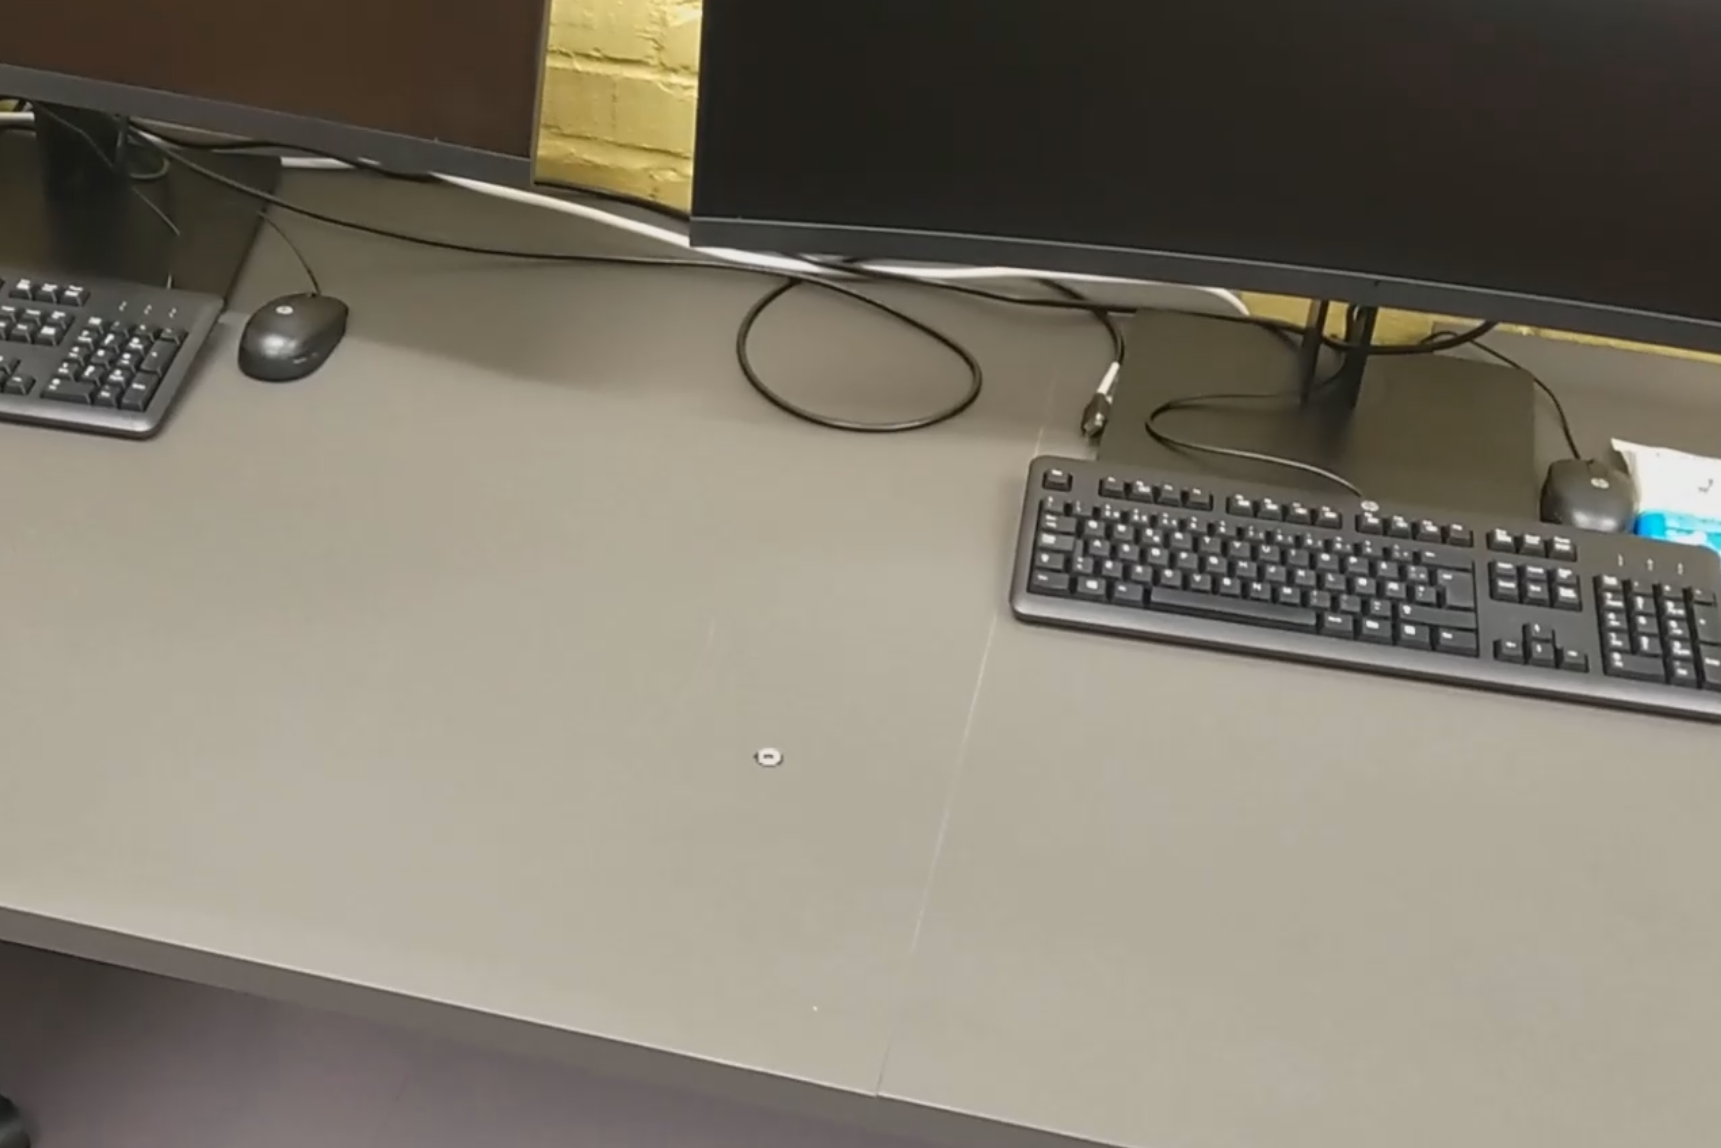
\includegraphics[width=0.5\textwidth]{fig/mvpdemo1.png}
    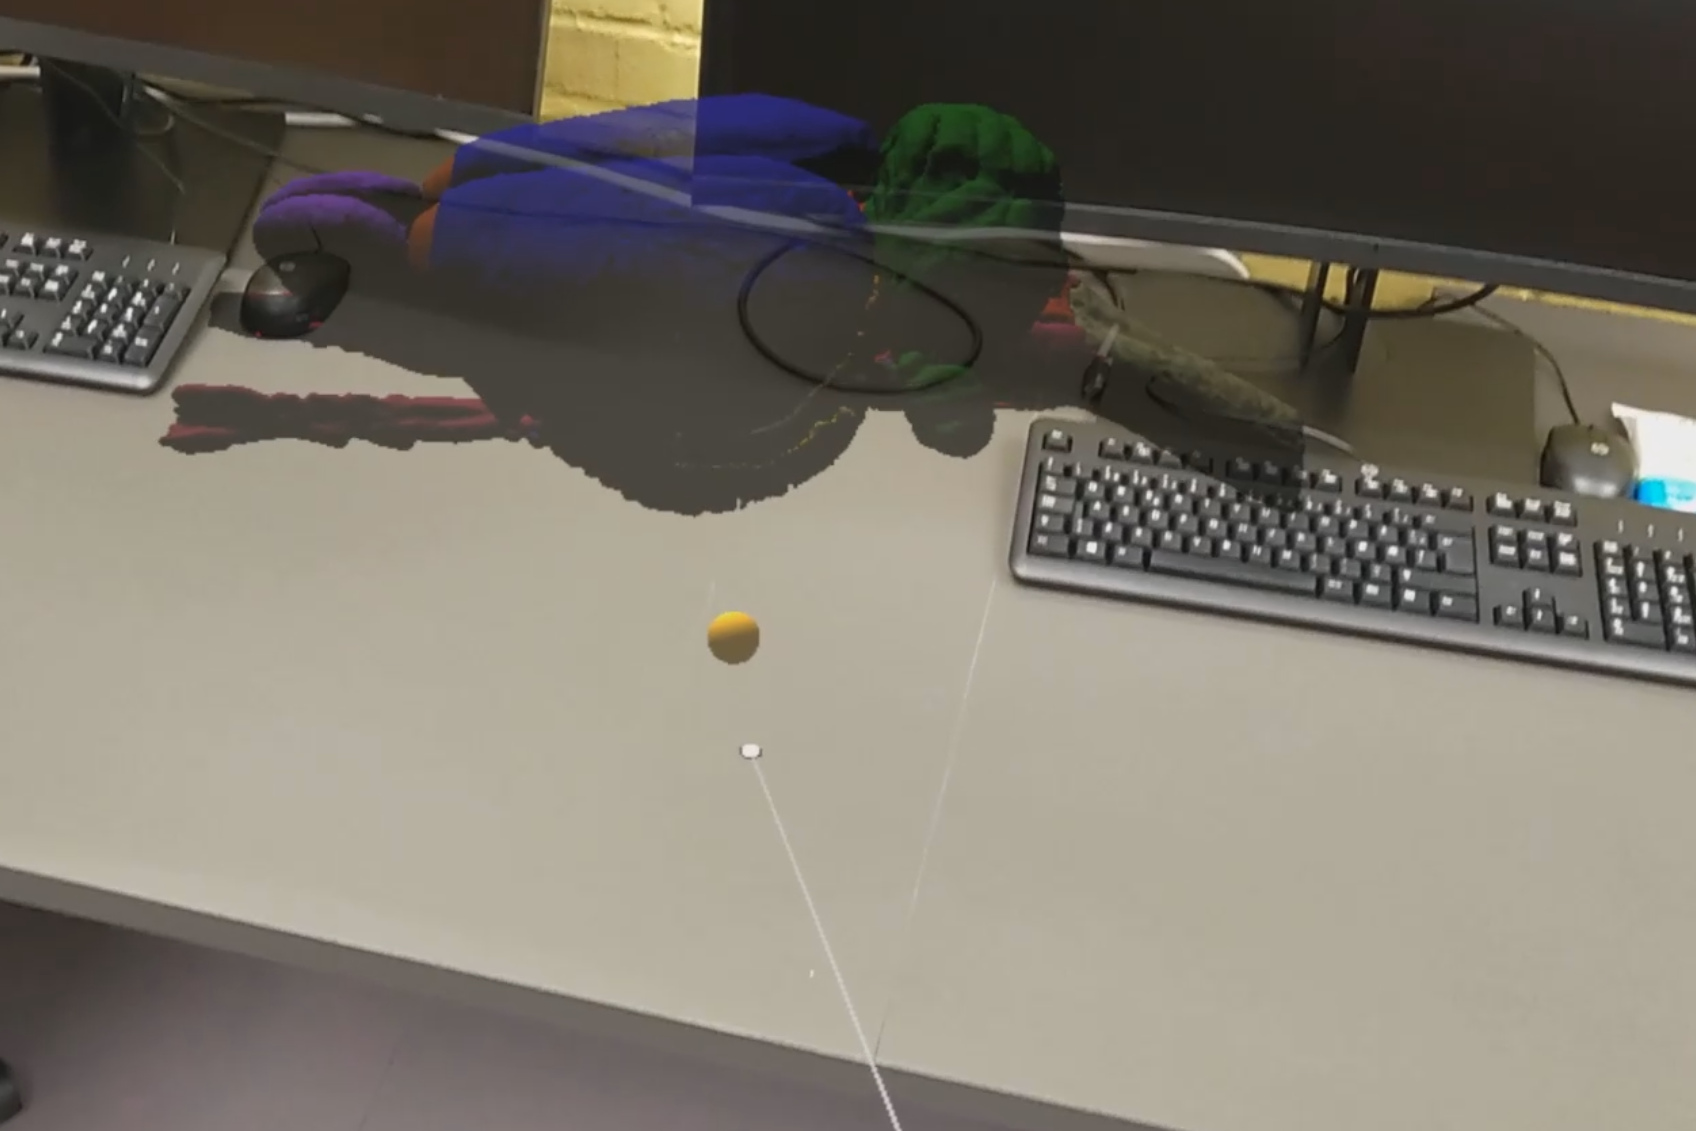
\includegraphics[width=0.5\textwidth]{fig/mvpdemo2.png}
    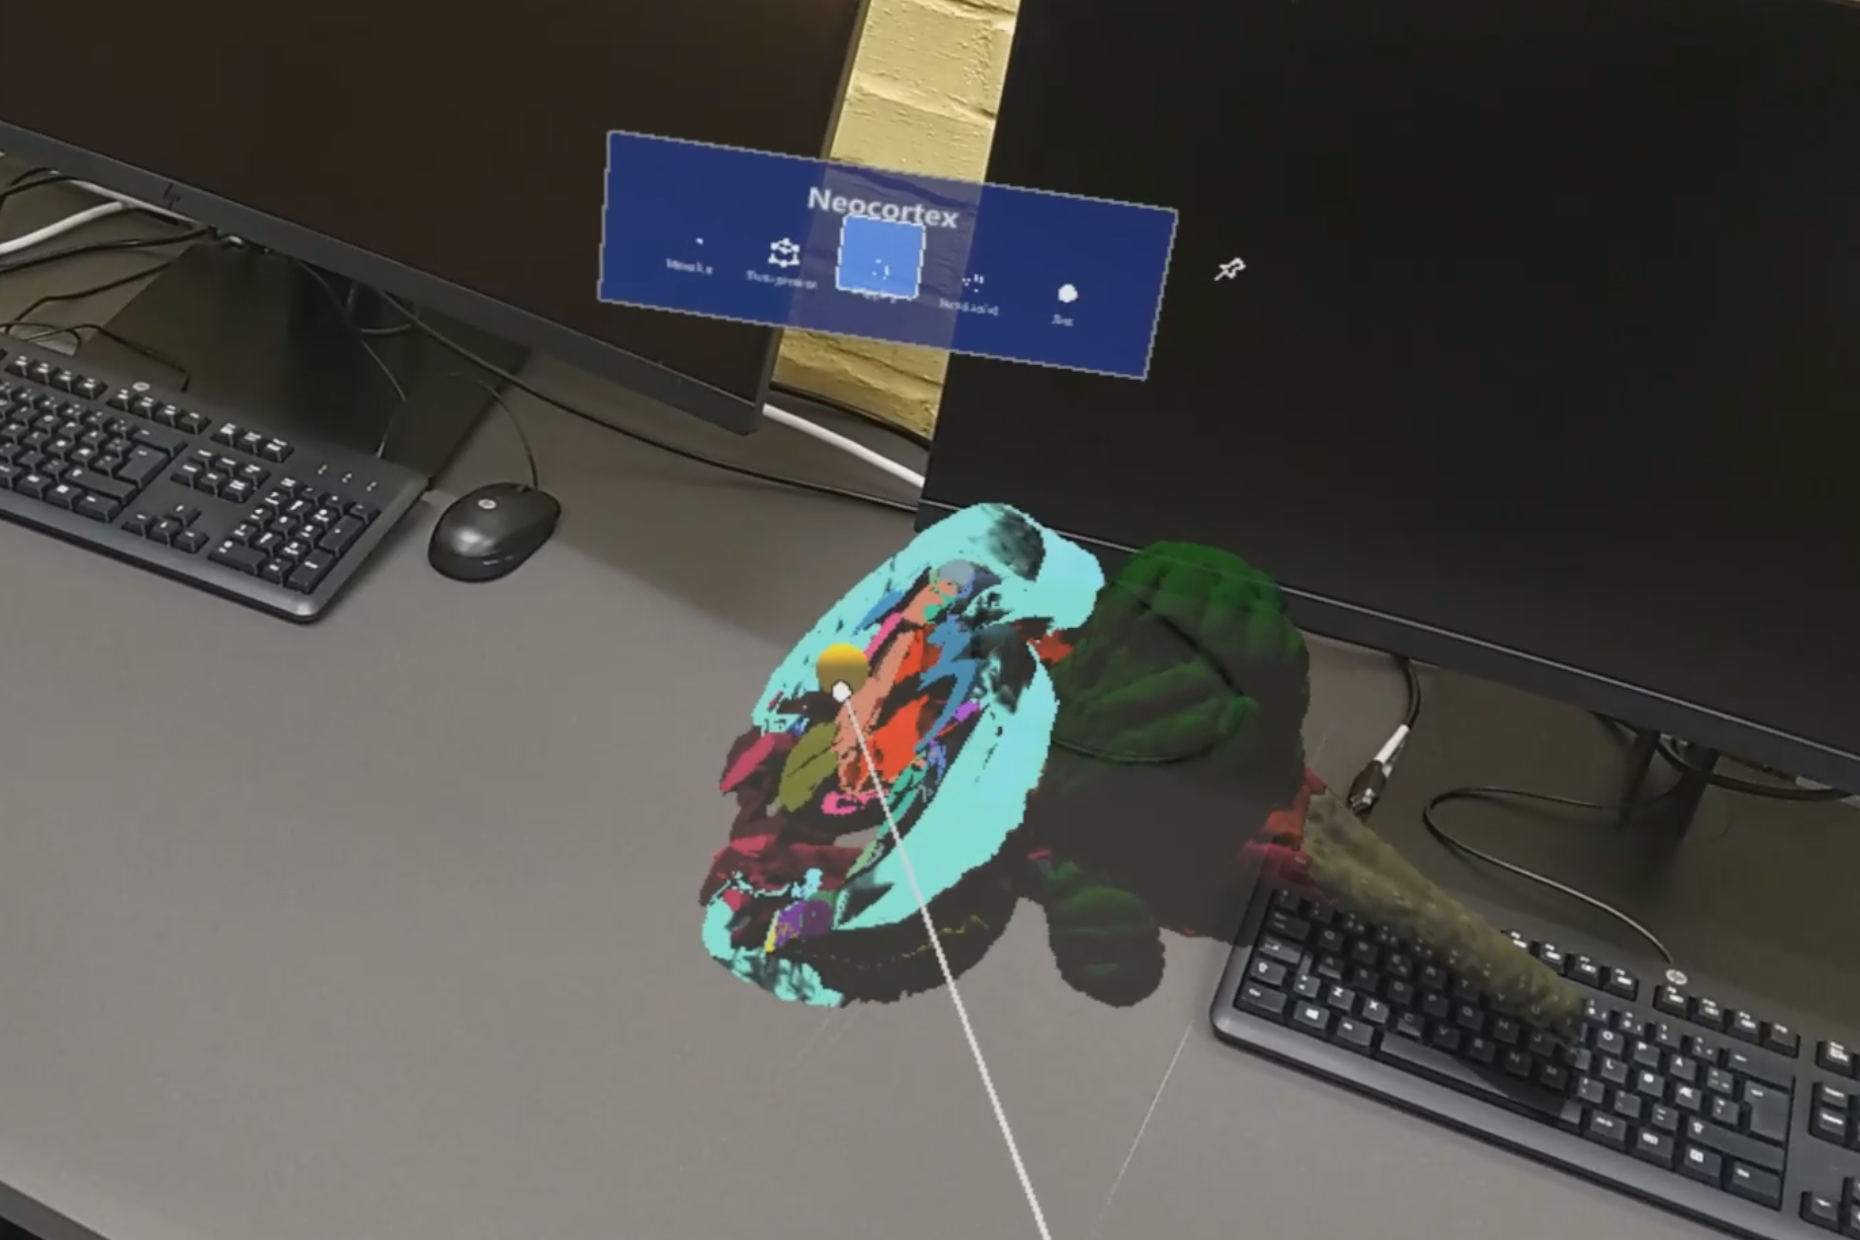
\includegraphics[width=0.5\textwidth]{fig/mvpdemo3.png}
    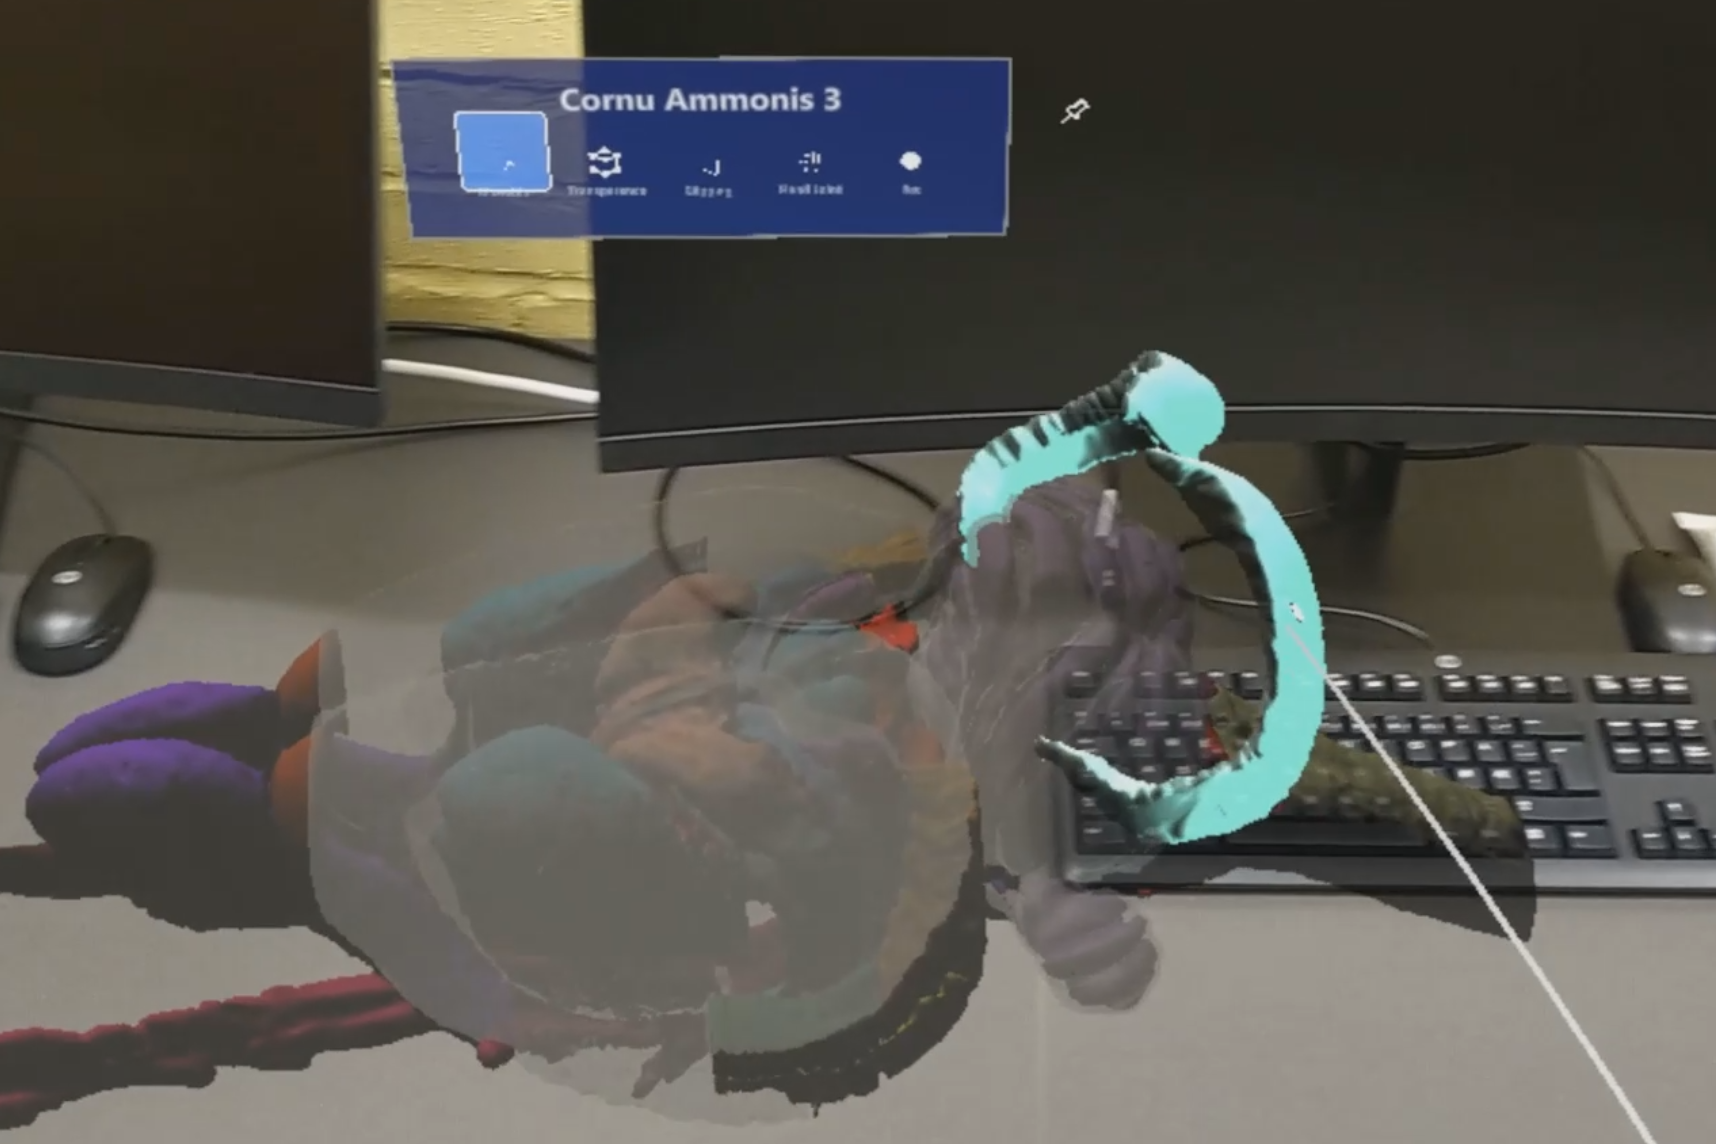
\includegraphics[width=0.5\textwidth]{fig/mvpdemo4.png}
    \caption{The first demo of the application, running on the HoloLens 2.}
    \label{fig:mvpdemo}
\end{figure}

\subsection[Iteration N]{Next iterations: Continuing development}

The continuation of the project will be explored further, but will focus on implementation of highlighted features and and high-level overview of the process, rather than a chronological log as in previous sections. 
% This section will give a overview of the continued progress in developing the application and highlighting some specific features. 

Shortly after end of the first iteration a demonstration of the application was done over video conference, with a pre-recorded YouTube video, demonstrating the features of the application. In addition a physical stakeholder meeting at St. Olavs Hospital was arranged where only the project researcher used the application with the HMD, but through live streaming the video feed from the headset and operational guidance from Dr. Menno Witter testing of dissection features were held. The application was at this stage nearly identical to what was seen at the end of the \nameref{chap:itr1}, with minor tweaks and bug fixes.

After this initial demonstrations stakeholders from the Kavli Institute were intrigued to see further development and had very positive sentiments toward the research project. Feedback gathered from this meeting included mainly two features, an ability to place brain structures back into the brain after deconstruction, basically to tidy up the brain after manipulation. Second, a list view for choosing which brain structures should be visible, this feature request was inspired by Eldens \nameref{chap:vrvis} which some of the stakeholders had previous experience with.

\subsubsection*{Snapping}
The first of the described feature request to be able to put brain structures back into place. Snapping structures as magnets was suggested as a metaphor for the action. 

This snapping effect was implement as a \texttt{MonoBehavior} called \texttt{SnapInPlace}, by storing the initial position of each snappable object and comparing the distance to this position with a given \texttt{snapThreshold} distance at the end of each manipulation: 

\begin{lstlisting}[language=c]
void OnManipulationEnded() {
    if (Distance(storedPosition, currentPosition) < snapThreshold) 
        currentPosition = storedPosition; 
}
\end{lstlisting}

This worked well enough, however no indication of the snapping behavior was given to the user and so it could be interpreted as an unexpected behavior when the brain structure just disappears when the user releases it. This issue was solved by having a semi-transparent shadow of the brain structure at its initial position colored green when snapping would occur at release and gray otherwise. Additionally, a audio effect was implemented such that a clicking sound as the structure snapping in place. 

\begin{figure}
    \centering
    % 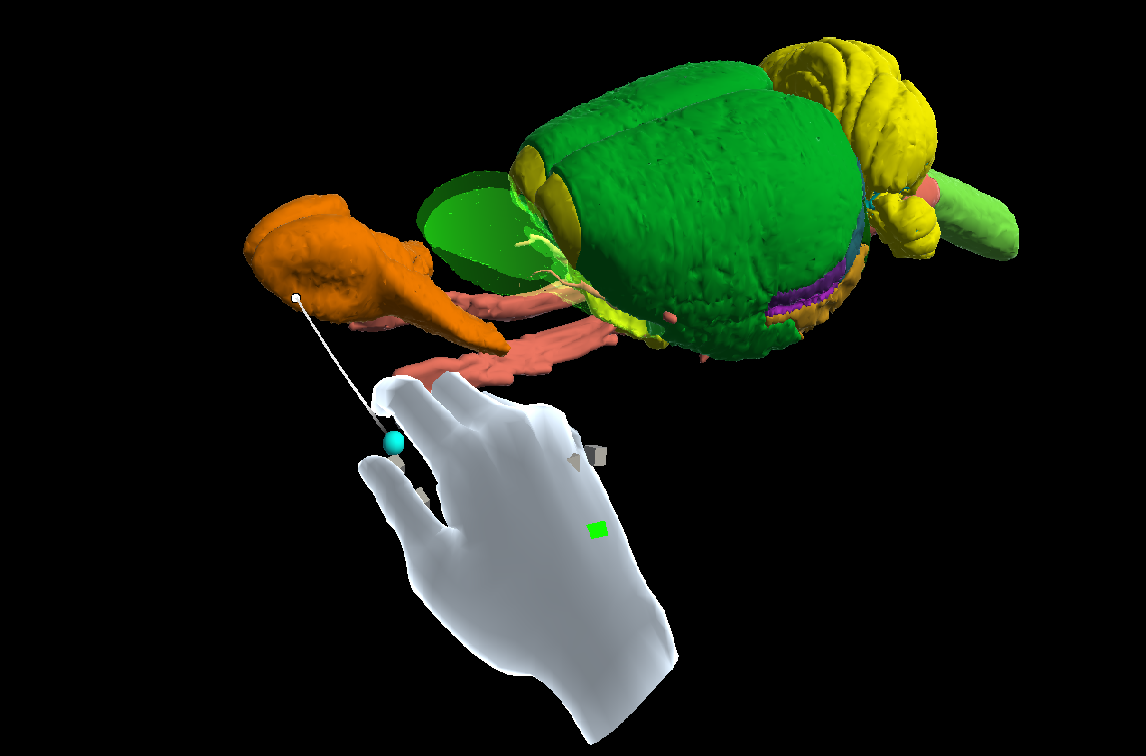
\includegraphics[width=0.65\textwidth]{fig/snaphint.png}
    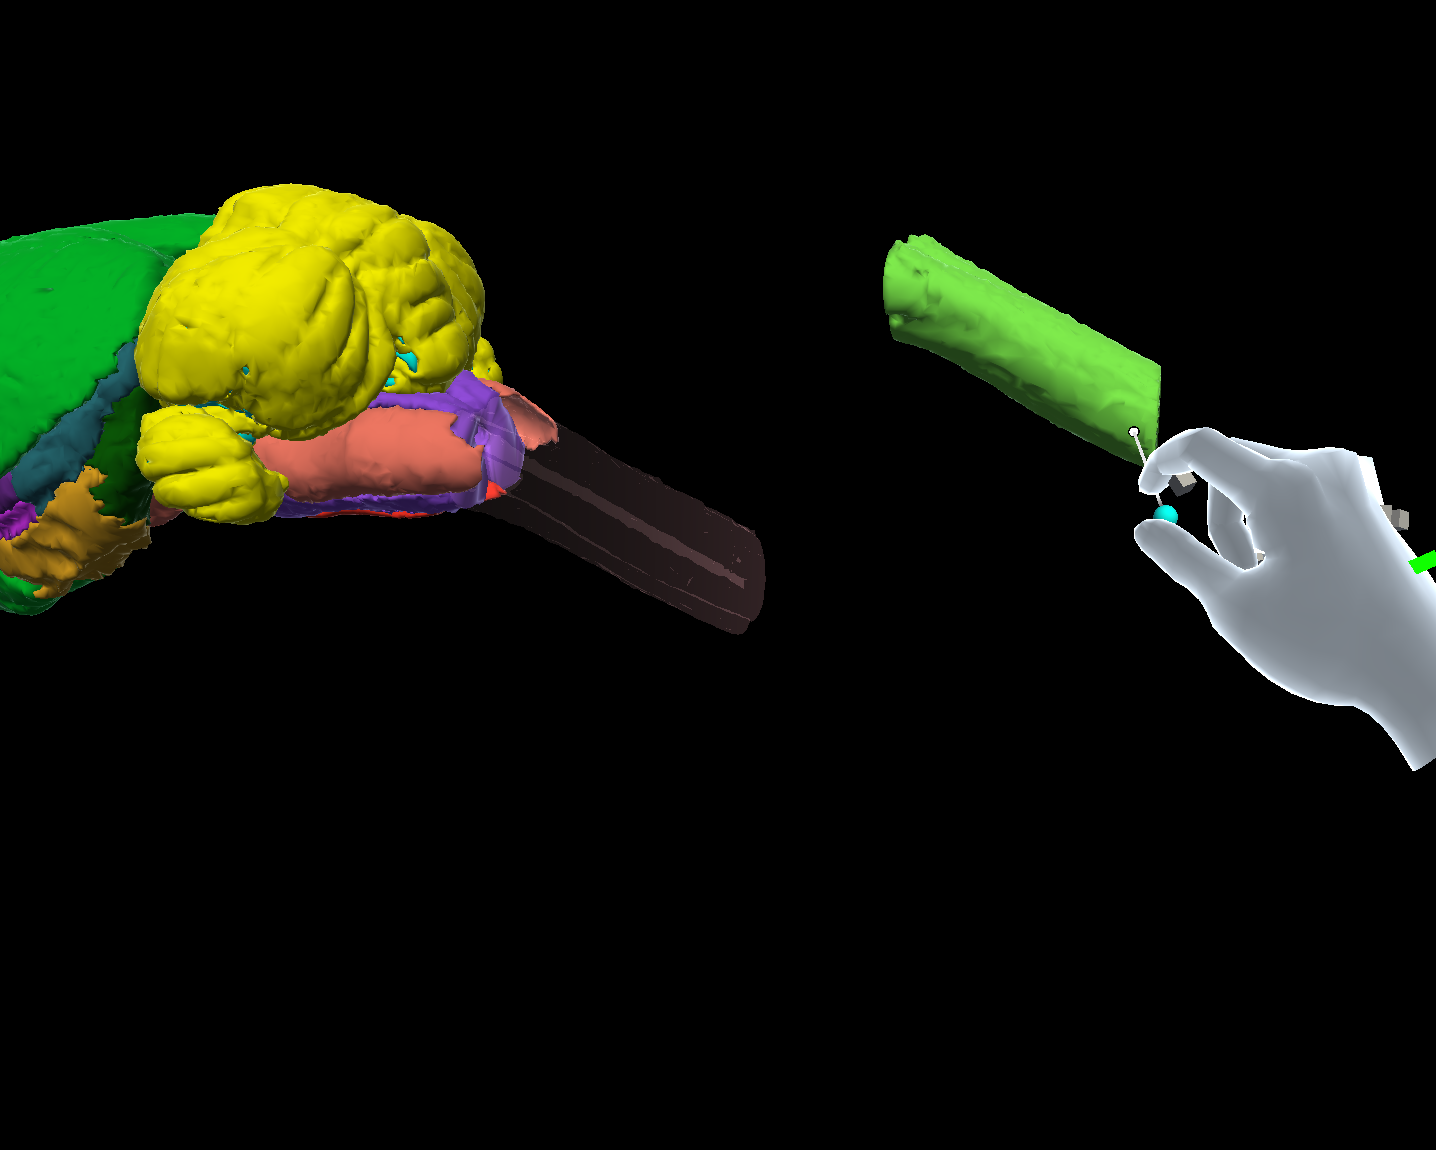
\includegraphics[width=0.32\textwidth]{fig/snaphint1.png}
    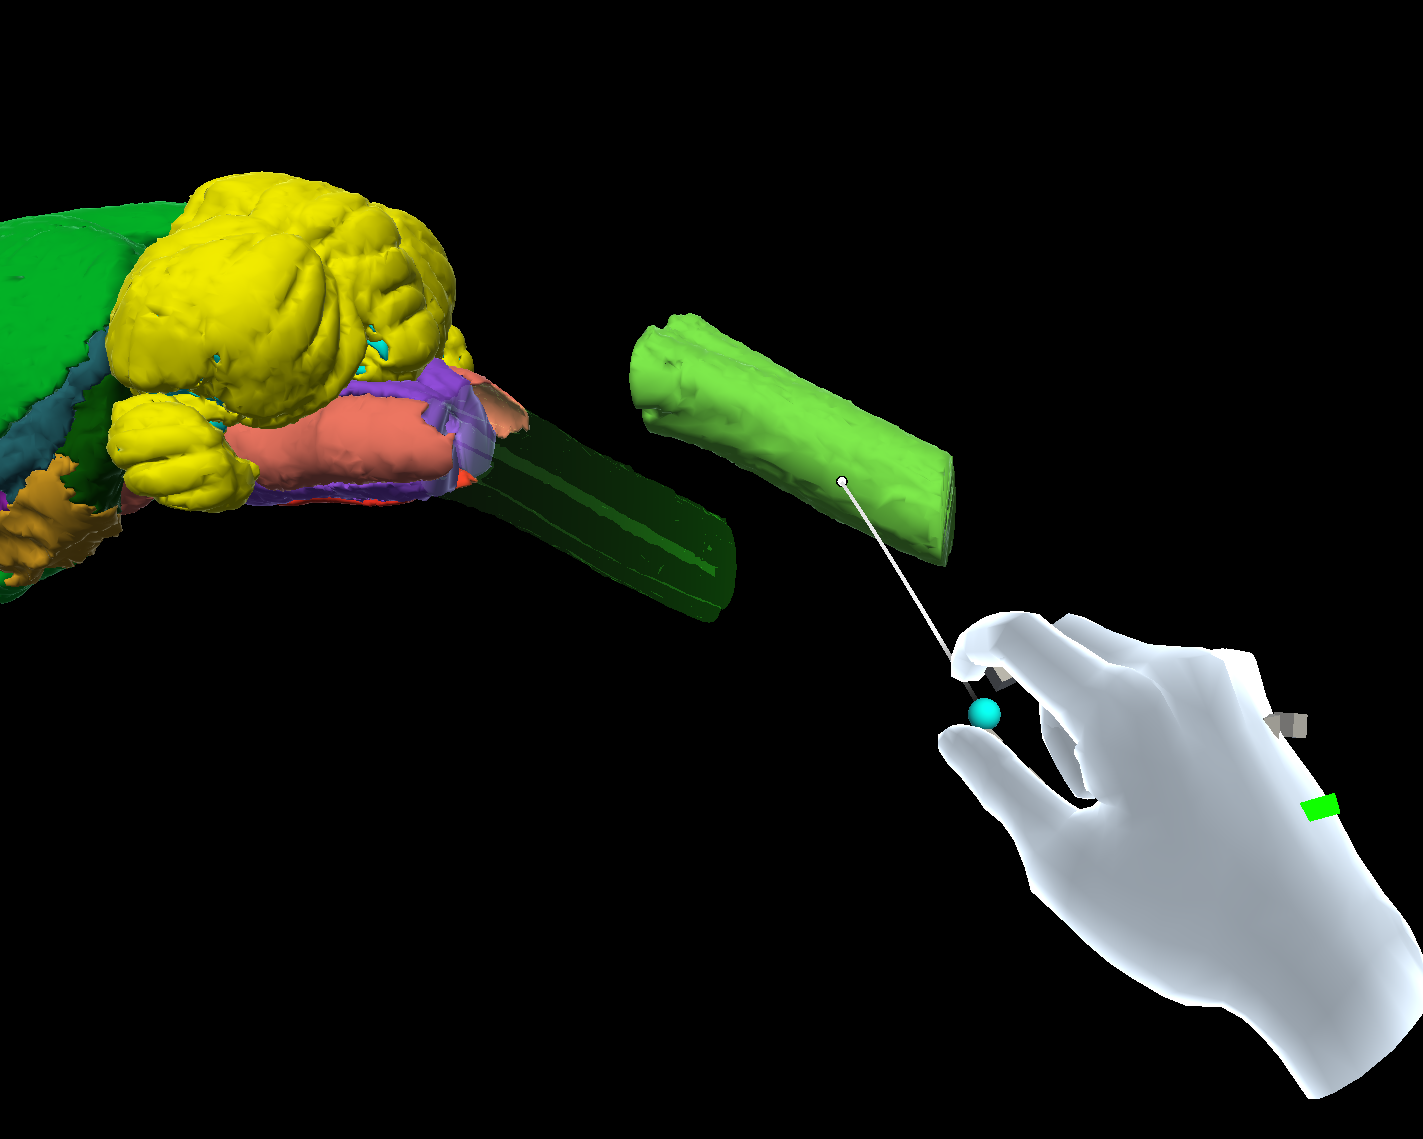
\includegraphics[width=0.32\textwidth]{fig/snaphint2.png}
    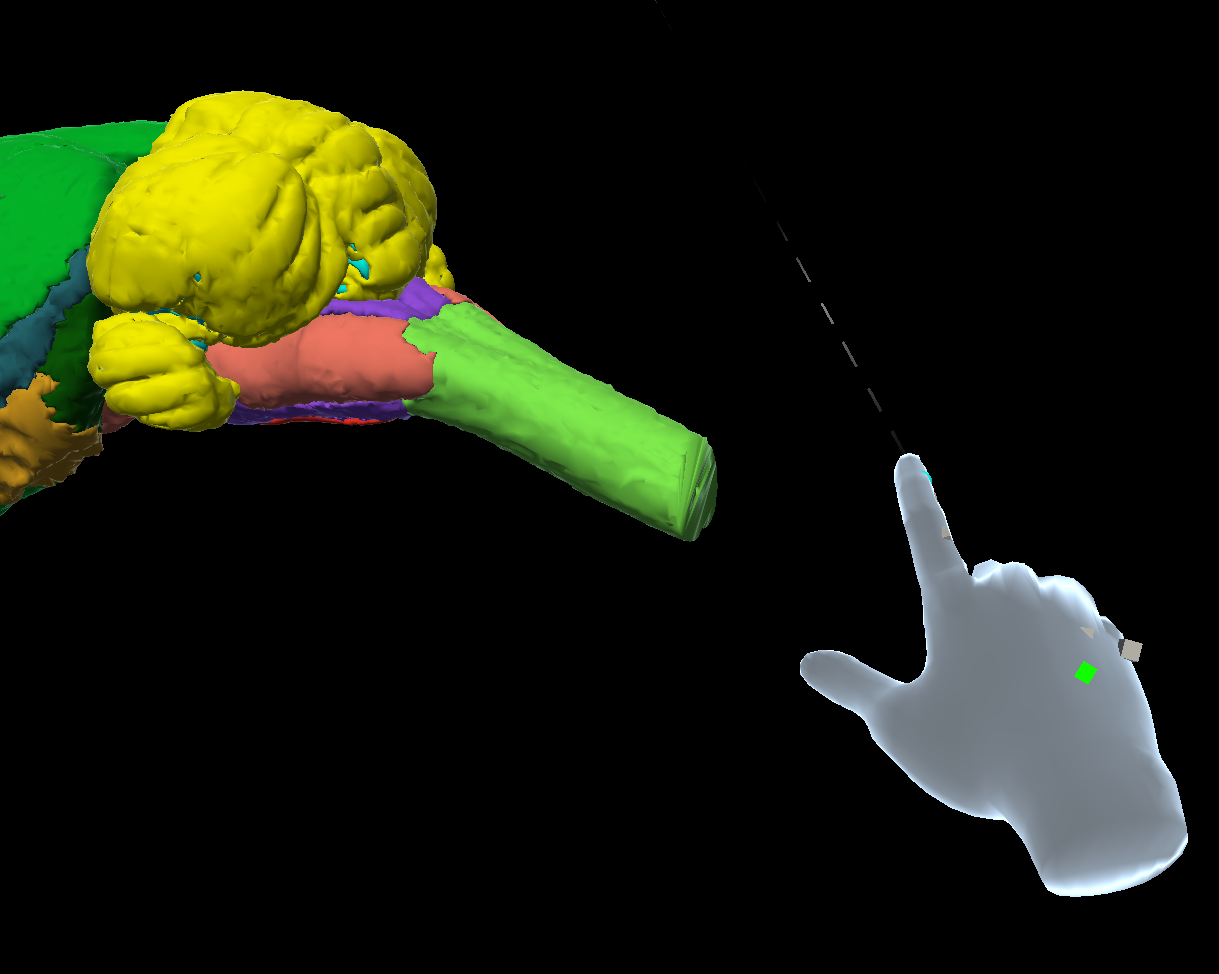
\includegraphics[width=0.32\textwidth]{fig/snaphint3.png}
    \caption{The complete snapping process. Right most image shows the brain structure snapping in place at release.}
\end{figure}

\subsubsection*{Scrollable list view}

A list view similar to the one in \nameref{chap:vrvis}, as seen in \autoref{fig:vrvis} was requested by stakeholders. 


\subsubsection*{UI, menus and stuff }


\subsubsection*{Feedback from demo}
% list view

\subsubsection*{Coloring brain}

\subsubsection*{Info Board}
Textual information about the brain structures was requested by stakeholders as a educational tool for student to use by them self or in groups. The idea was that lecturers could add text as they see fit and change it to an appropriate level for the intended user group. 
This feature was implemented based on the MRTK \texttt{Slate} with is an AR based floating text box, perfect to simulate a black board. In fact, if wished for in the future it would be trivial to make it look more as a black board by changing the color and the font to something more handwritten.
The slate was customized by changing the content text reference from \texttt{InfoBoard} MonoBehavior when the a new brain structure was selected, this was done with a \texttt{UnityEvent}, a simple callback function, implemented to trigger when a new brain section is selected (this implementation
 is found in \texttt{NetworkBrainManager.cs}). The text descriptions for each structure is saved as a text file and is parsed in \texttt{InfoBoard.cs}, the text file uses a custom structure where "@" at the begin of a line indicates a new brain structure and "+" indicates a added images and and all other text is seen as descriptions for the last indicated brain structure. This works well enough, but an obviously more standard and readable approach would be to use a common text based serialization format like JSON or XML. In future development it should be looked into using one of these as both are well supported with built-in deserialization features in Unity with C\#. The implementation does not support any run-time importing of this text even though the parsing is done at run time, functional it would thus be trivial to add. What has to be implemented for this to work however is either file exploring or some other way of accessing files, e.g. from network, see \nameref{chap:futurework} for more on this.

\subsubsection*{Clustering}

By clustering brain structures based on the neurological attributes lecturers can visualize how complete compound structures operation and where they are located in the brain. Just as the \texttt{InfoBoard} this feature utilizes a custom text file parser to define each clusters name, brain structures and color pallet. Again JSON or XML would probably be a wise transition for these configuration files. 
When selecting the clustering action, the \texttt{Clustering} MonoBehavior iterates through all brain structures and enables or disables according to whether it is a part of the cluster. It also assigns a new color based on the color pallet defined in the configuration file. Color pallets are defined based on HSV color hues, with two numbers indicating start and end hue in degrees, then the brain structures are assigned colors uniformly the given sector of the color wheel. This was found to be a simple and reliable solution to color coding, but could with ease be argue as not being a intuitive solution for unaccustomed or non-technical users. 
For users not to loose spatial orientation when exploring the clusters a outline of the rat brain was added. This outline is a hollow version of the geometric brain model, which was created by manually selecting all outer vertices of the brain model using Blender, this is far from a perfect approach and gives a inaccurate and rough outline and a high polygon count, however if not for future performance issues the author sees no need to fix this.


\begin{figure}[h]
    \centering
    % 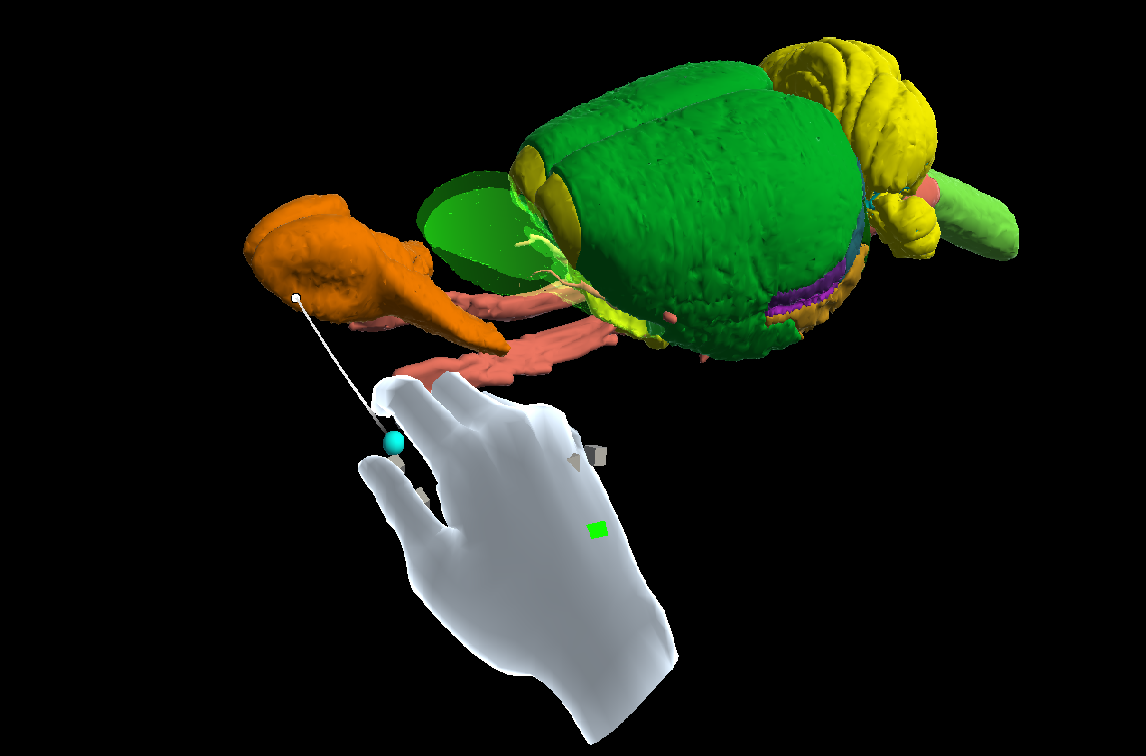
\includegraphics[width=0.65\textwidth]{fig/snaphint.png}
    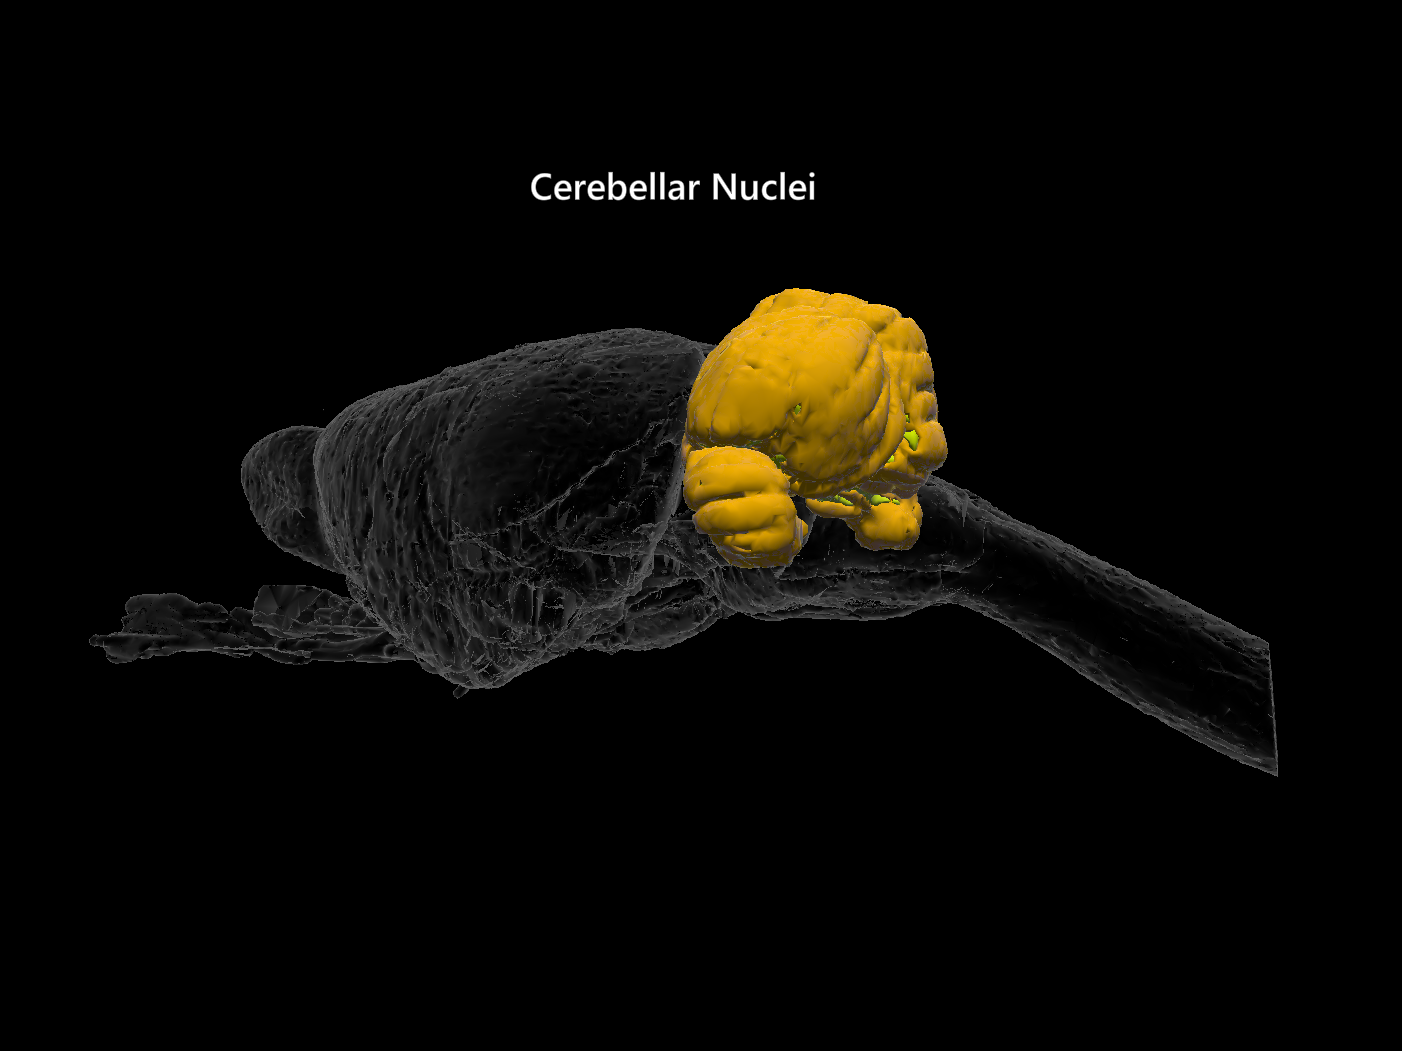
\includegraphics[width=0.32\textwidth]{fig/cluster1.png}
    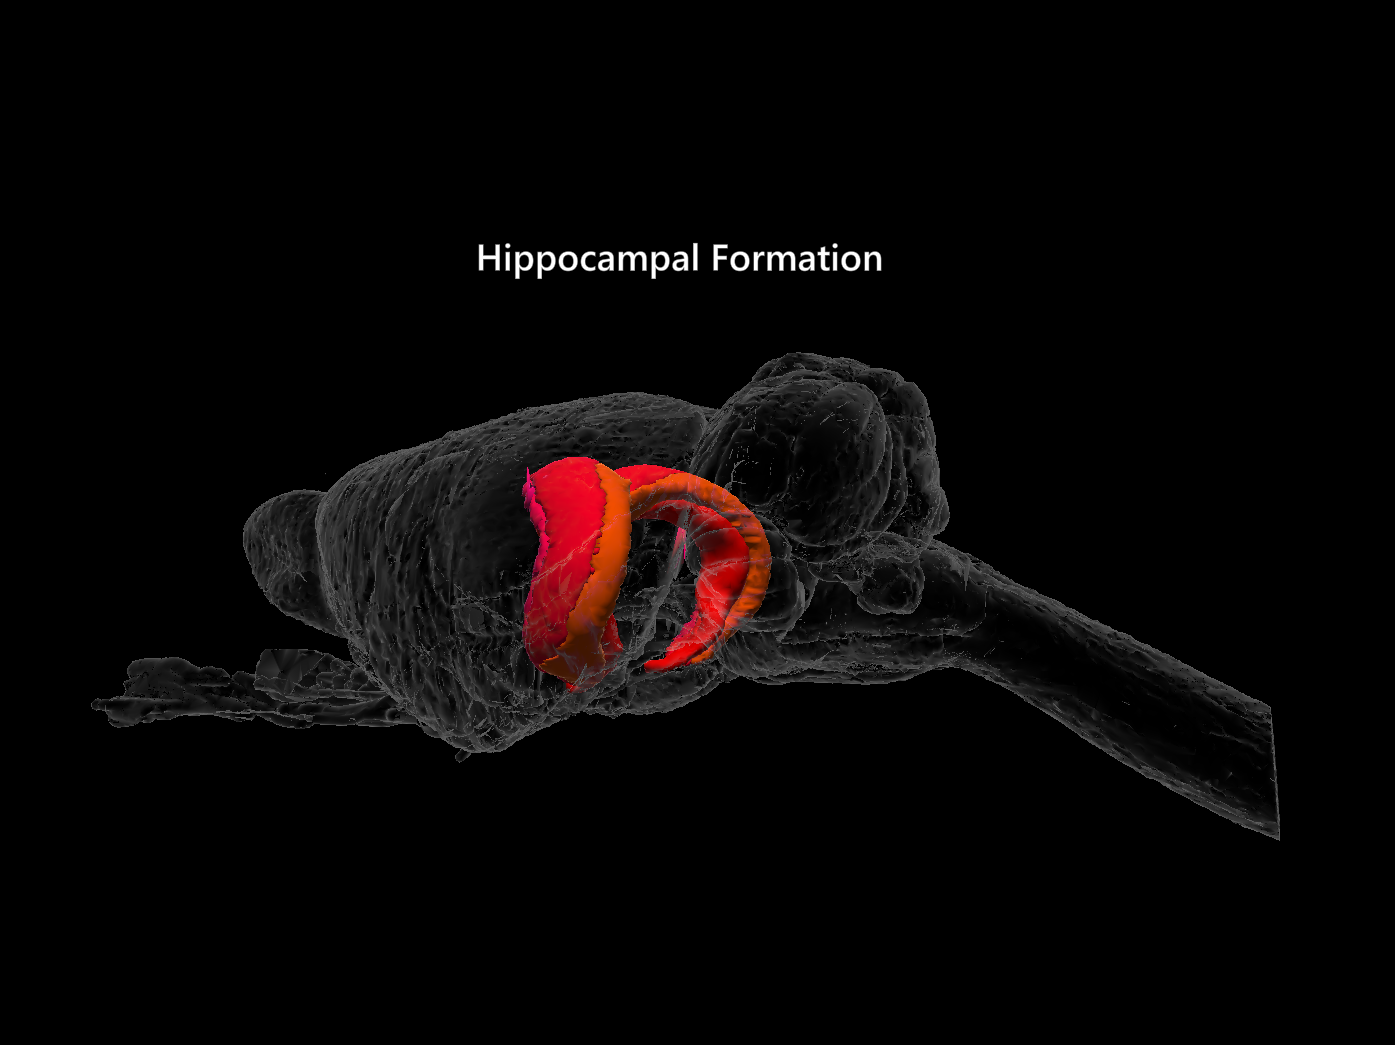
\includegraphics[width=0.32\textwidth]{fig/cluster2.png}
    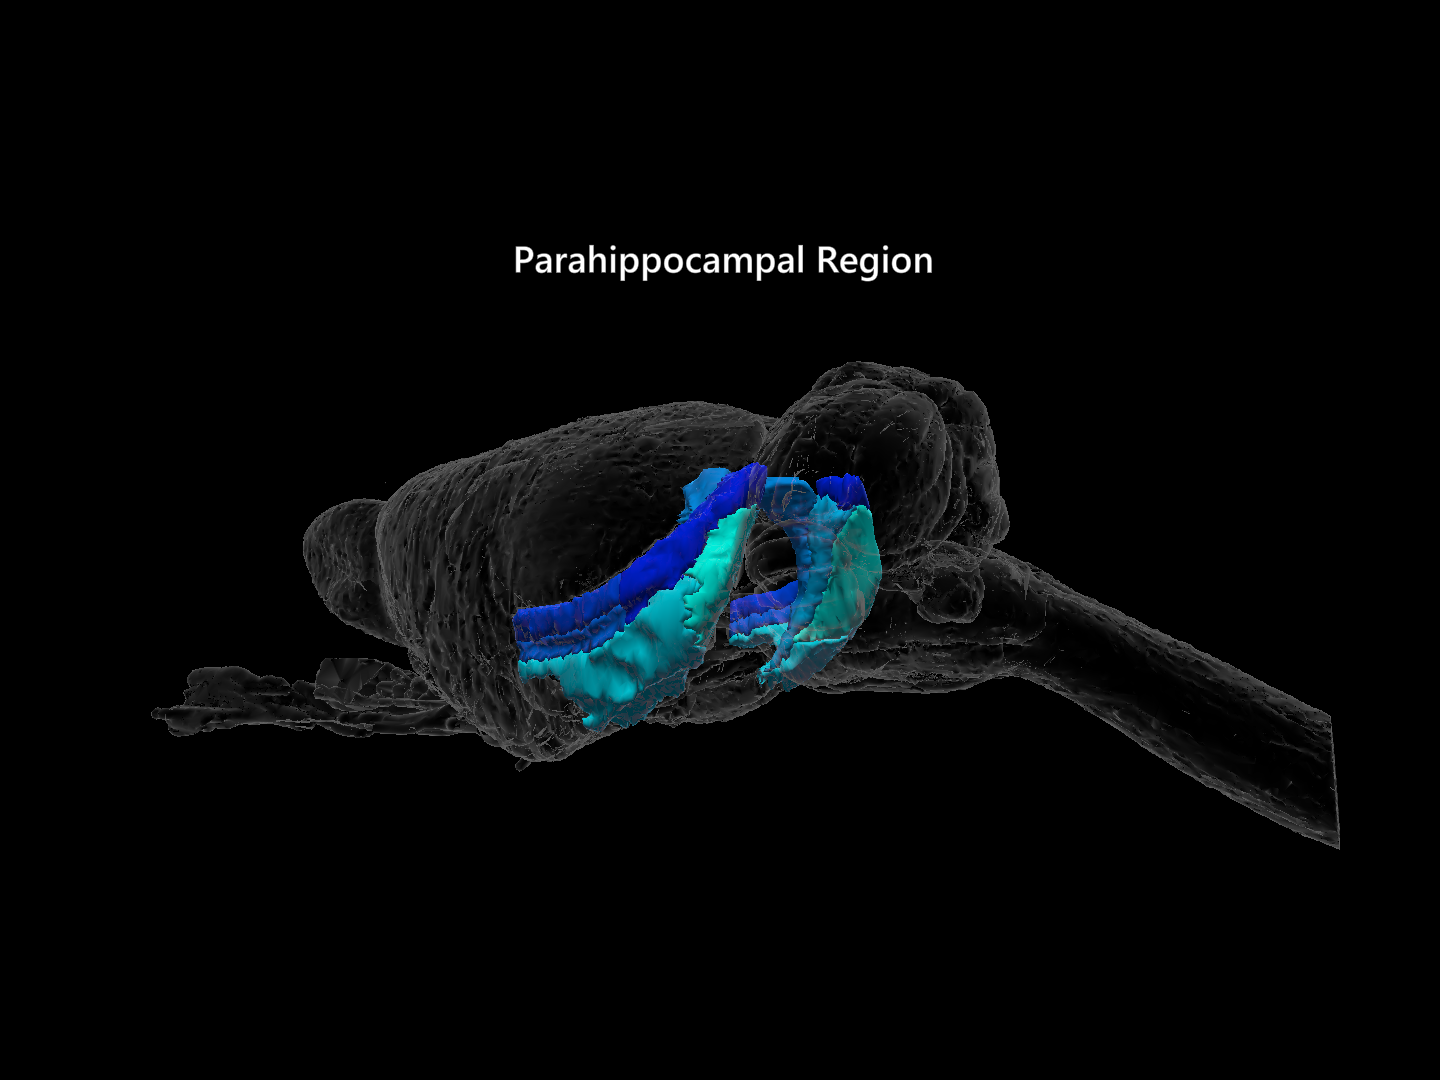
\includegraphics[width=0.32\textwidth]{fig/cluster3.png}
    \caption{Clusters in Nevrolens.}
\end{figure}


\subsubsection*{Porting to Android}
% The application was originally developed for HoloLens 2, but other platforms were always in mind and because of the use of \nameref{chap:mrtk}, deploying to other platform was relatively easy, within the documentation for MRTK, there was guides for how to build for Android. Interaction on Android is more complicated though. Because all interaction happens on screen additional effort has to be laid down to implement a good user experience on smartphone.  

As MRTK is a framework specifically designed for HoloLens development, the HoloLens 2 naturally became the main focus of development and thus the application running on Android is a porting of the HoloLens version with small changes to somewhat accommodate the smartphone interface. It has however seen too little platform specific development and is in reality an incomplete product. It is however very much usable and can be seen as a great demonstration of the multiplatform capabilities of MRTK. 
Porting to Android was initially done by simply deploy the same application to Android, this is easily done in Unity with some MRTK tweaks which can be read up on in the \href{https://microsoft.github.io/MixedRealityToolkit-Unity/version/releases/2.2.0/Documentation/CrossPlatform/UsingARFoundation.html}{documentation}. While this works, some expected features are missing. For example, on the HoloLens 2 the user enables actions in a menu which is bound to their hand this is not possible in Android because the user interacts with the application not by moving the hand in space, but by touching the devices screen, therefore the application will simply disable the hand following feature on Android such that the menu buttons are static in space at all time. This is far from a optimal solution, but has worked for basic proof of concept. 
\begin{lstlisting}[language=c]
if (runtimePlatform != GlobalSettings.SupportedPlatform.HoloLens2)
{
    GetComponent<HandConstraintPalmUp>().enabled = false;
}
\end{lstlisting}

% There are of course some 


\subsubsection*{Volumetric dissection plane}





\subsubsection*{Networking optimization}

\subsubsection*{}



% \subsection*{3rd iteration: Implementing network}
\subsection[Final Iteration]{Final Iteration}\label{chap:finaliter}









